\subsection{LowProFool} % 概要
表形式データに対する敵対的サンプルの生成手法として,Balletらが提案したLowProFool\cite{ballet2019imperceptible}がある.表形式データの特徴として識別に寄与する各特徴量の重要度が異なることが多い.LowProFoolはこの点に着目し各特徴量の重要度を元データから算出し,それに基づいたノイズを付加することで誤分類を引き起こし,検知されにくい敵対的サンプルを生成する.

% LowProFoolの問題設定
LowProFoolは検知されにくい敵対的サンプルを生成するため,以下の最適化問題を解く.
\autoequation{\bm{r}^* = \mathrm{arg}_{\bm{r}} \min d(\bm{r}) \text{ for } \bm{r} \in \mathbb{R}^D}
\autoequation{\text{s.t. }  f(\bm{x}) = s \neq f(\bm{x}+\bm{r}^*) = t,  \bm{x}+\bm{r}^* \in A}

式(2)は最適化を式(3)は制約を表している.
式(2)における $d(\bm{r})$ は式(4)のように定義される.
\autoequation{d_{\bm{v}}(r) = ||\bm{r} \odot \bm{v}||^2_p}
各特徴量の重要度を考慮するため,ノイズベクトル $\bm{r}$ と特徴量重要度ベクトル $\bm{v}$ のアダマール積 $\odot$ を用い,その大きさを $\ell_2$ ノルムで評価する.また,ノイズベクトル $\bm{r}$ は元データと同じ $D$ 次元の実数空間から選ばれる.
式(3)の一つ目の制約 $f(\bm{x}) = s \neq f(\bm{x}+\bm{r}^*) = t$ は,元データ $\bm{x}$ の分類結果 $s$ とノイズを付加したデータ $\bm{x}+\bm{r}^*$ の分類結果 $t$ が異なることを要求する.二つ目の制約 $\bm{x}+\bm{r}^* \in A$ は,生成された敵対的サンプルが現実的な値域 $A$ に収まることを保証する.$A$ は,元データから各特徴量に対する最小値から最大値の集合であり,元データの分布を大きく崩さないようにするために用いられる.

% 目的関数について
上記の最適化問題を解くため,以下の目的関数は式(5)を定義する.

\autoequation{g(r) = L(\bm{x}+\bm{r}, t) + \lambda ||\bm{v} \odot \bm{r}||_2}

 目的関数は,二つの項から構成される.第一項 $L(\bm{x}+\bm{r}, t)$ は損失関数であり,元データ $\bm{x}$ にノイズ $\bm{r}$ を付加したデータを誤分類させたい目標ラベル $t$ に分類させることを目的としている.第二項 $\lambda ||\bm{v} \odot \bm{r}||_2$ は,特徴量重要度ベクトル $\bm{v}$ を用いてノイズの検知されにくさを制御している.ここで第二項にはバランスを調整するパラメータ $\lambda$ がある.
 これにより,元データの特徴量の重要度を考慮しつつ,検出されにくい敵対的サンプル $\bm{x}'$ を生成する.

次にLowProFoolのアルゴリズムを示す.アルゴリズムの各ステップは以下の通りである.
\begin{algorithm_step}
    \item[Step 1)] アルゴリズムで使用する変数の初期化を行う.ノイズベクトル $\bm{r}$ を
        ゼロベクトルで初期化する.また,初期サンプル $\bm{x}_0$ を元のサンプル $\bm{x}$ とする.
    
    \item[Step 2)] 最大反復回数 $N$ まで以下の計算を繰り返す.まず,前述の目的関数 
        $g(r) = L(\bm{x}+\bm{r}, t) + \lambda ||\bm{v} \odot \bm{r}||_2$ の勾配を計算する.
        次に,計算された勾配に基づいてノイズベクトル $\bm{r}$ を更新する.
        更新されたサンプルが有効な値域に収まるようクリッピングを行う.
    
    \item[Step 3)] 最適な敵対的サンプルの選択を行う.生成された敵対的サンプルの中から,
        元のサンプルとは異なるクラスに分類される($f(\bm{x}_i) \neq f(\bm{x}_0)$)ことと,
        検知されにくさの指標 $d_v(\bm{x}_i)$ が最小となるものを選ぶ.
    
    \item[Step 4)] 選択された敵対的サンプル $\bm{x}'$ を返す.
    \end{algorithm_step}


このアルゴリズムの特徴は,各反復において特徴量の重要度を考慮しながらノイズを更新する点にある.重要度の高い特徴量に対しては小さな摂動に抑えられ,重要度の低い特徴量により大きな摂動が許容される.これにより,分類結果を変更しつつも,検知されにくい敵対的サンプルの生成が可能となる.
また,クリッピング操作により,生成されるサンプルが常に有効な値域に収まることが保証される.例えば,年齢のような非負の特徴量が負の値を取ることを防ぐことができる.


\subsection{特徴量の重要度算出方法}

前述の通り,識別に寄与する特徴量を考慮した上で,ノイズを付加する.特徴量重要度 $\bm{v}$ の算出は,分類結果に対する各特徴量の相関係数を用いることが提案されていた.ピアソンの相関係数を用いて以下のように定義される.

\autoequation{\bm{v} = \cfrac{|\rho_{\bm{X},Y}|}{\|\rho_{\bm{X_i},Y}\|^2_2}}
ここで,$d$ は特徴量の次元数,$\|\rho_{\bm{X},Y}\|$ は $i$ 番目の特徴量 $\bm{X_i}$ と目的変数 $\bm{Y}$ の相関係数を示している.各特徴量と目的変数の関係性の強さを示す指標であり,値が大きいほどその特徴量が分類結果に寄与していることを意味する.また,分母は全ての特徴量の寄与度の二乗和の平方根を表し,全体の相関のスケールに対して分子を正規化している.これにより,特徴量重要度 $\bm{v}$ は,各特徴量が持つ相関の相対的な重要性を反映した値となる.この特性により,上記のアルゴリズムでは最小化を行うため,相関係数が大きい特徴量に対しては小さなノイズが付加されることになり,重要度を表現することができる.今回のデータセットによって生成された特徴量重要度を算出した図を下に示す.

\begin{figure}[H]
    \centering
    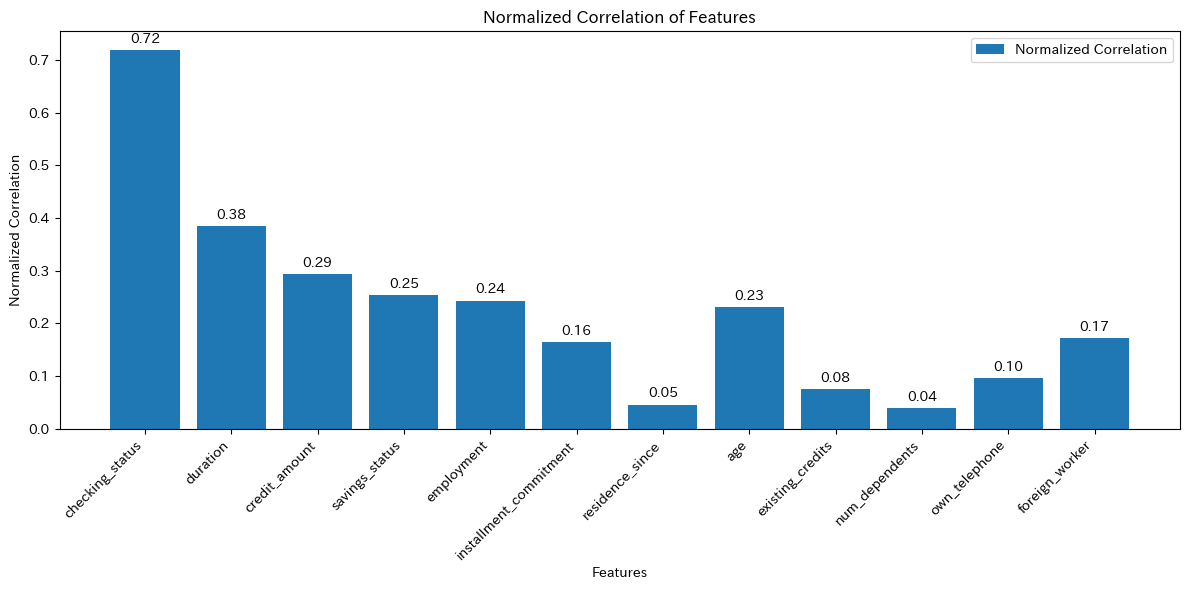
\includegraphics[width=0.8\textwidth]{images/従来手法_特徴量重要度.png}
    \caption{従来手法:各特徴量における重要度}
    \label{fig:default_method_feature_importance}
\end{figure}


\subsection{従来手法の課題}
従来手法を使用し,敵対的サンプルを生成した.生成された敵対的サンプルの一例を以下に示す.


生成された敵対的サンプルを確認すると以下の課題が見られた.

一つ目に特定の特徴量に対するノイズが集中してしまっていることをも挙げられる.特徴量重要度の算出方法において,相関係数が大きい特徴量に対してノイズを大きく避けるため,次に重要な特徴量へのノイズ集中してしまっている可能性がある.よって明らかに不自然に大きいノイズを抑えるような特徴量重要度の算出が重要になっている.
    

二つ目に,敵対的サンプルの出力が連続値であることが挙げられる.今回使用するデータセットは前述の通り特徴量が全て離散値である.敵対的サンプルが連続値を取ることで,離散値を持つ特徴量に対して生成された敵対的サンプルが現実的でない値をとってしまっている.このため,連続値の敵対的サンプルを離散値に変換する必要がある.


これらの課題に対して,次節では改良手法を提案する.